% Kopfzeile beim Kapitelanfang:
\fancypagestyle{plain}{
%Kopfzeile links bzw. innen
\fancyhead[L]{\calligra\Large Vorlesung Nr. 23}
%Kopfzeile rechts bzw. außen
\fancyhead[R]{\calligra\Large 14.01.2013}
}
%Kopfzeile links bzw. innen
\fancyhead[L]{\calligra\Large Vorlesung Nr. 23}
%Kopfzeile rechts bzw. außen
\fancyhead[R]{\calligra\Large 14.01.2013}
% **************************************************
%
\wdh
\enum{
\item Integration der Treppenfunktion 
\\*
(leicht)
\item $f: [a, b] \to \R$ beschränkt\\
$\int_a^b {}_* f(x) = sup \left\lbrace \int_a^b g(x)dx \vert g: [a,b] \to \R Treppenfunktion, g \leq f \right\rbrace$\\*
$inf \left\lbrace \int_a^b h(x)dx \vert h: f\ \leq h \right\rbrace = \int_a^b {}^* f(x)$
%\begin{tikzpicture}[domain=0:2,prefix=plots/, smooth]
%\draw[very thin,color=gray] (-0.3,0.0) grid (2.5,2.0);
%\draw[->] (-0.3,0) -- (2.5,0) node[right] {$x$};
%\draw[->] (0,-0.3) -- (0,2) node[above] {$y$};
%\draw[color=black] plot[id=23.2_int] function{cos(x)+1} node[below, midway] {$f(x)$};
%%\draw[color=green] (0, 2) -- (0.5, 2);
%%\draw[color=green] (0.5, 2) -- (0.5, 1.87);
%%\draw[color=green] (0.5, 1.87) -- (1, 1.87);
%%\draw[color=green] (1, 1.87) -- (1, 1.54);
%%\draw[color=green] (1, 1.54) -- (1.5, 1.54);
%%\draw[color=green] (1.5, 1.54) -- (1.5, 1.07);
%%\draw[color=green] (1.5, 1.07) -- (2, 1.07);
%%\draw[color=green] (2, 1.07) -- (2.5, 1.07);
%%\draw[color=green] (2.5, 1.07) -- (2.5, 0.2);
%%\draw[color=green] (2.5, 0.2) -- (3, 0.2);
%%\draw[color=green] (3, 0.2) -- (3.5, 0.1);
%\end{tikzpicture}\\*
$f$ \ul{integrierbar} wenn $\int_a^b{}_* f(x)dx=\int_a^b{}^* f(x)dx$, dann $\int_a^b f(x)dx:=\int_a^b{}_* f(x)dx$
\enum{
\item $f:[a,b]→\R$ stetig \Rarr\ integrierbar
\item Mittelwertsatz: Wenn $f:[a,b]→\R$ stetig, dann gibt es ein $x_0 \in [a,b]$ mit $\int_a^b f(x)dx=f(x_0)·(b-a)$\\*
(Grundlage aller Berechnungen) %Graph mit fläche
}
}
\uS{Hauptsatz der Differential und Integralrechnung}
\sS{Satz}
Sei $I\subseteq\Re$ Intervall, $f:I→\R$ stetige Funktion, $a\in I$ feste Zahl.\\*
Definiere: $$F(x):=\int_a^x f(t)dt$$
(Erinnerung: Wenn $x<a$, dann $\int_a^x\underset{Def}{=}=-\int_x^a$)\\*
Dann ist $F:I→\R$ \ul{differenzierbar} und $F'(x)=f(x)$.
\bew
Sei $h≠0$ $$\frac{F(x+h)-F(x)}{h}=\frac{1}{h}\left(\int_a^{x+h}f(t)dt-\int_a^xf(t)dt\right)=\frac{1}{h}\int_a^{x+h}f(t)dt$$\\*
% Treppengraph, erste Tafel
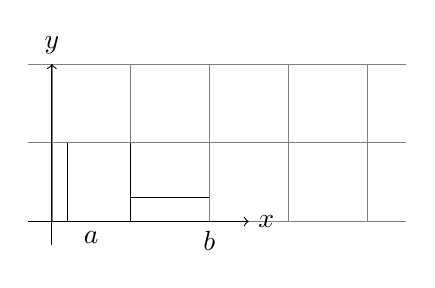
\begin{tikzpicture}
\draw[very thin,color=gray] (-0.3,0.0) grid (4.5,2.0);
\draw[->] (-0.3,0) -- (2.5,0) node[right] {$x$};
\draw[->] (0,-0.3) -- (0,2) node[above] {$y$};
\draw (0.5,0) node[anchor=north] {$a$};
\draw (2,0) node[anchor=north] {$b$};
% Schrafierung einfügen
\draw (0.2, 1) -- (0.2, 1);
\draw (0.2, 0) -- (0.2, 1);
\draw (1, 0) -- (1, 1);
\draw (1, 0.3) -- (2, 0.3);
\end{tikzpicture}\\*
Mittelwertsatz \Rarr\ es gibt $x_h\in[x,x+h]$ (wenn $h>0$) bzw. $x_h\in[x+h,x]$ (wenn $h<0$), so dass
%$$\int_a^{x+h}f(t)dt=f(x_n)·h\ \Rarr\ (*) = \frac{f(x_n)·h}{h}=f(x_n)\ \Rarr\ F'(x)=\lim_{h→0}\frac{F(x+h)-F(x)}{h}=\lim_{h→0}f(x_n)\underset{\footnote{\text{Für $h→0$ ist $x_n→x$, denn $|x-x_n|\leq h$, $f$ \ul{stetig}}}}{=}f(x)\ \Rarr \text{Behauptung}$$\qed

\sS{Definition Stammfunktion}
Sei $f:I→\R$ Funktion. Eine Funktion $F:I→\R$ heißt Stammfunktion von $f$ wenn $F$ Differenzierbar und $F'=f$\\*
\bem
9.9 \Rarr\ Jede stetige Funktion $f$ hat eine Stammfunktion

\sS{Satz}
Sei $F$ Stammfunktion von $f$\\*
Eine Funktion $G:I→\R$ ist Stammfunktion von $f$ \equ\ $F-G$ konstant, dass heißt $G=F+c$ mit $c\eR$
\bew
$G$ differenzierbar mit $G'=f$ \equ\ $G-F$ differenzierbar mit $(G-F)'=f-f=0$ \equ\ $G-F$ konstant (bekannt)\qed

\sS{Satz (Hauptsatz der Differenzial und Integralrechnung)}
%Sei $f:[a,b]→\R$ stetig, $F:[a,b]→\R$ Stammfunktion von $f$, dann $$\int_a^{b} f(x)dx=F(b)-F(a)=:F(x) \vert\alg{b\\a}$$
\bew
Sei $G(x):=\int_a^xf(t)dt$, $G:[a,b]→\R$.\\*
9.9 \Rarr\ $G'=f\ \underset{9.11}{\Rarr}\ G-F=c$ konstant, $c\eR$. $G=F+c$
$$\int_a^bf(x)dx=G(b)=G(b)-\underbrace{G(a)}_{=0}=F(b)+c-(F(a)+c)=F(b)-F(a)$$\qed\\*
\sss{Folge} Berechnung von Integralen \equ\ Finden von Stammfunktionen = Umkehrung des Ableitens
\notat{"$\int f(x)dx=F(x)$"(*)}
soll heißen: $F$ ist Stammfunktion von $f$, dass heißt $F'=f$\\*
Vorsicht: (*) ist keine echte Gleichung, bestimmt $F(x)$ nur bis auf Addition einer Konstante
\bsp
Sei $s\in\R\setminus\{-1\}$ $\ds\int_a^b x^s dx$\\*
Erlaubter Interpretationsbereich: \\*
% Graph an der dritten Tafel mit schrafur.
\begin{tikzpicture}[domain=0.5:2,prefix=plots/, smooth]
\draw[very thin,color=gray] (-0.3,0.0) grid (2.5,2.0);
\draw[->] (-0.3,0) -- (2.5,0) node[right] {$x$};
\draw[->] (0,-0.3) -- (0,2) node[above] {$y$};
\draw (0.5,0) node[anchor=north] {$a$};
\draw (2,0) node[anchor=north] {$x-h$};
\draw (0.5, 0) -- (0.5, 1.5);
\draw (2,0) -- (2, 0.6);
\draw[color=blue] plot[id=23.1_int2] function{sin(2x+0.5)} node[below, midway] {};
\end{tikzpicture}\\*
\enum{
\item $s \eN$: $a,b$ beliebig
\item $s \eZ$: $s\leq -2:\ x=0$ ausschließen $x^s = \frac{1}{x^{-s}}$ entweder $a,b < 0$ oder $a,b > 0$
\item $s \in \R \setminus \Z$\\*
$x^3 := e^{3 \cdot log (x)}$ nur definiert für $x > 0$
$a, b > 0$
Suche $F$ mit $F' = x^s$\\*
$F=\frac{1}{s+1} x^{s+1}$ $F' = (s+1) \frac{1}{s + 1} x^2 = s^2$\\*
$s \neq -1 \Rarr s+1 = 0$\\*
$\int_a^b $ % NOOB
Für uns nur die Reste.
}
\bsp
\enum{
\setcounter{enumi}{1}
\item{$\int e^x dx = e^x$, denn $(e^x)'=e^x$}
}
%\item $\int sin(x)dx=-cos(x) denn (-cos(x))'=sin(x)$\\*
%$\int cos(x)dx=sin(x) denn (sin(x))'=cos(x)$
%(Unbestimmte Integrale) \underset{z.B.}{\Rarr} $\Int_a^b e^xdx=e^x\left|\alg{b\\a}\right.=e^b-e^a$ etc.
%$$\int e^{cx}dx=\frac{1}{c}e^{cx}\qquad\frac{1}{c}(e^{cx})'=\frac{1}{c}·c·e^{cx}=e^{cx}$$
%$$\int x^sdx, s≠1 …\text{ bekannt aus 1)}$$
%\item $$\int_a^b x^{-1} dx = \int_a^b \frac{1}{x} dx$$
%% Graph f(x) = 1/x
%Erlaubte Grenzen: $x \neq 0$\\*
%d.h. $a, b > 0$ oder $a, b < 0$
%\itm{
%\item Sei $a, b > 0\quad$. $log'(x) = \frac{1}{x}\quad$ $\log: \R_0 \to \R$\\*
%\Rarr{} $\int_a^b \frac{1}{x}dx = log(x) \mid^b_a$ wenn $a, b > 0$
%\item Sei $a, b < 0$ Sei $g: \R_{<0} \to \R$, $g(x) = log(-x) = log(|x|)$\\*
%$g'(x) = \frac{1}{-x} \cdot (-1) = \frac{1}{x}$\\*
%$\int_a^b \frac{1}{x} = log(-x) \mid_a^b = log(|x|) \mid_a^b$
%}
%In beiden Fällen:
%$\int \frac{1}{x}dx = log(|x|)$ wenn $x \neq 0$
%\item{ $\int\frac{1}{1+x^2}dx=arctan(x)$\\*
%GRAPH fehlt noch
%\bew
%$tan=\frac{sin}{cos}:[-\frac{\pi}{2},\frac{\pi}{2}]→\R$\\*
%$(tan(x))'=\frac{1}{cos(x)^2}$\\*
%% GRAPH
%Wenn $y=tan(x)\qquad arctan'(y) = \frac{1}{tan'(x)}=cos(x)^2 \overset{!}{=} \frac{1}{1+y^2}$
%$$cos(x)^2 \overset{!}{=} \frac{1}{1+\frac{sin(x)^2}{cos(x)^2}}=\frac{cos(x)^2}{cos(x)^2+sin(x)^2}=cos(x)^2$$\ok
%}


Grundprinzip:\\*
Jede Ableitungsregel gibt eine Integrationsregel:
\itm{
\item Kettenregel $\to$ Substitutionsregel
\item Produktregel $\to$ Partielle Integration
}

\uS{Substitutionsregeln}
\sS{Satz}
Sei $f:I→\R$ stetig, $\phi:[a,b]→I$ differenzierbar, dann $$\int_a^b f(\phi(t))·\phi'(t)dt=\int_{\phi(x)}^{\phi(b)}f(x)dx$$
\bew
Sei $F:I→\R$ Stammfunktion von $f$, dass heißt $F'=f$
%$$(F·\phi)'(x)=F'(\phi(x))·\phi'(x)=f(\phi(x))·\phi'(x)\ \Rarr \int_{\phi(x)}^{\phi(b)}f(x)dx=F(x)\left|\alg{\phi(b)\\\phi(a)}\right.=F(\phi(b)-F(\phi'(a))$$
$F(\phi(X)) \mid_a^b = \int_a^b (F(\phi \circ F)'(x)) dx = \int_a^b f(\phi (x)) \cdot \phi'(x)dx$
\bsp
\enum{
\item $\int_a^b f(x + c)dx = \int_a^b \underbrace{f(\phi(t))}_f(t+c) \cdot \underbrace{\phi'(t)}_{=1} dt) = \int_{a + c}^{b + c} f(x) dx$\\*
$\phi(t) = t + c$
$\phi'(t) = 1$
\item $\int_a^b f(c \cdot x) = \int_a^b f(\phi(t)) \cdot \frac{\phi'(t)}{c}dt = \frac{1}{c} \cdot \int_a^b f(x) dx$
\item $$\Int_a^b t:f(t^2)dt=\footnote{$\phi(t)=t^2\quad\phi'(t)=2t$}\frac{1}{2}\Int_a^b\underbrace{\phi'(t)}_{2t}·f(\phi(t))=\frac{1}{2}\Int_{a^2}^{b^2}f(x)dx$$
z.B. $\Int_0^1xe^{x^2}dx=\frac{1}{2}\int_{0^2}^{1^2}e^xdx$ \\*
%$f(x)=e^x=\frac{1}{2}e^2\left|\alg{1\\0}\right.=\frac{e-1}{2}$
$F(\phi(X)) \mid_a^b = \int_a^b (F(\phi \circ F)'(x)) dx = \int_a^b f(\phi (x)) \cdot \phi'(x)dx$
}
\bsp
\enum{
\item $\int_a^b f(x + c)dx = \int_a^b \underbrace{f(\phi(t))}_f(t+c) \cdot \underbrace{\phi'(t)}_{=1} dt) = \int_{a + c}^{b + c} f(x) dx$\\*
$\phi(t) = t + c$
$\phi'(t) = 1$
\item $\int_a^b f(c \cdot x) = \int_a^b f(\phi(t)) \cdot \frac{\phi'(t)}{c}dt = \frac{1}{c} \cdot \int_a^b f(x) dx$
}
%$f(x)=e^x=\frac{1}{2}e^2\vert\alg{1\\0}=\frac{e-1}{2}$
